\documentclass[sigconf]{acmart}

\input{format/final}

\begin{document}
  \title{Comparing Predictive Models of Pain Reliever Misuse and Abuse}
  \author{Sean M. Shiverick}
  \affiliation{
  \institution{Indiana University-Bloomington}
  }
\renewcommand{\shortauthors}{S.M. Shiverick}

%%%%%%%%%%%%%%%%%%%%%%%%%%%%%%%%%%%%%%%%%%%%%%%%%%%%%%%%%%%%%%%%%%%%%%%%%%%%%%%%

\begin{abstract}

The misuse and abuse of prescription opioids (MUPO) has become a major health 
crisis in the U.S. The rise of opioid overdose deaths in recent years is also 
correlated with the increased availability of illicit and synthetic opioids
\cite{nida18}. Predictive models can be used to identify demographic factors 
related to MUPO and may help predict individuals at risk for opioid addiction.
The present study compares several linear and non-linear classification models 
of pain reliever misuse and abuse to identify the models that best fit the data. 
The sample data consisted of N = 114,038 respondents from the National Survey 
on Drug Use and Health (NSDUH) from 2015 and 2016. Classification models 
vary in terms of complexity, accuracy, and interpretability. 

Simple models provide interpretable solutions but may have lower accuracy 
than more complex models which provide higher accuracy but are often more 
difficult to interpret.   

\footnote{ Address correspondence to \textit{smshiver@iu.edu}}
\end{abstract}
\keywords{Predictive Modeling, Supervised Learning, Classification Models}
\maketitle

%%%%%%%%%%%%%%%%%%%%%%%%%%%%%%%%%%%%%%%%%%%%%%%%%%%%%%%%%%%%%%%%%%%%%%%%%%%%%%%%
\section{Introduction}

The misuse and abuse of prescription opioids (MUPO) over the past two 
decades has become a major health crisis in the U.S. \cite{volkow14}. 
An estimated 2 million Americans suffered a substance use disorder related 
to prescription opioid pain relievers such as oxycodone or hydrocodone 
in 2015 \cite{nida18}. Opioid dependence and relapse are chronic health 
conditions and following treatment many addicted individuals are at high 
risk for relapse and overdose death \cite{shaham03}. From 1999 to 2016, 
the number of opioid-related overdose deaths has more than quadrupled. 
On average, more than 115 people die from an opioid overdose each day 
\cite{cdc18, judd16}. Supply-based interventions to reduce the availability 
of prescription opioids have produced a shift to the use of heroin and 
synthetic opioids such as fentanyl \cite{jones15}. The dosage levels and 
potency of illicit and synthetic opioids are largely unknown which has
increased the risk of overdose death. The sharp rise in prescription 
overdose deaths (POD) and heroin overdose deaths (HOD) are correlated 
\cite{muhuri13, unick13}. Predictive analytics is a useful approach for 
modeling the variables that contribute MUPO. The present study compares 
several predictive models of pain reliever misuse and abuse to identify 
the models that best fit the sample data, and understand features that 
contribute to the misuse and abuse of prescription opioids.  

%%%%%%%%%%%%%%%%%%%%%%%%%%%%%%%%%%%%%%%%%%%%%%%%%%%%%%%%%%%%%%%%%%%%%%%%%%%%%%%%

\subsection{National Survey on Drug Use and Health} 

In the era of ``big data'', vast amounts of information are being generated 
from electronic medical records (EMRs), clinical research data, and population
-level health data \cite{hay13, herland14} that could provide insight to the
crisis of opioid misuse and addition. The data for the present study was 
obtained from the National Survey on Drug Use and Health (NSDUH) 
\cite{samhsa18}, a large comprehensive public survey with over 2600 variables
related to a diverse array of substance use, misuse, abuse, and dependency,  
including alcohol, tobacco, prescription medications and illicit drugs. 
The NSDUH also includes a complete set of demographic features including
physical health, depression, mental health treatment, and and substance 
abuse treatment. The public use data files of the NSDUH use a weighted 
sampling design across states by population size for a representative 
distribution that draws more heavily from the eight states with the largest 
population (e.g., CA, FL, IL, MI, NY, OH, PA, TX), accounting for 48 percent 
of the total U.S. population aged 12 or older. 

 The It can be difficult to obtain reliable 
information about drug usage based on self-reports   \cite{varshney13};
however, Survey research provides data on a wide range of issues that people 
may be reluctant to disclose, including mental health disorders, personal 
medical concerns, use of prescription medications, and illicit drug use. 
The target variable was individuals who reported misusing or abusing 
prescription pain medications at any point. The predictor variables of 
interest were select demographic variables, medication use, and use of 
illicit drugs (e.g., heroin, cocaine, amphetamines). The study goal was to 
construct and compare different predictive classification models to predict 
pain reliever misuse and abuse. Classification models were compared in order 
to select the best predictive models for the question under consideration,
the misuse and abuse of prescription opioids. 

%%%%%%%%%%%%%%%%%%%%%%%%%%%%%%%%%%%%%%%%%%%%%%%%%%%%%%%%%%%%%%%%%%%%%%%%%%%%%%%%
\subsection{Predictive Modeling}

Predictive modeling, statistical learning, or machine learning is a set 
of procedures and automated processes for extracting knowledge from data 
\cite{james13, kuhn13, muller17, raschka17}. The two main branches of 
predictive modeling are supervised learning and unsupervised learning. 
Supervised learning problems involve prediction about a specific target 
variable or outcome of interest. If a given dataset has no target outcome, 
unsupervised learning methods (e.g., clustering) can be used to discover 
underlying structure in unlabeled data. The present study uses a supervised 
learning approach to classify sample data as instances of pain reliever 
misuse and abuse (or not) and compare the performance of several different 
predictive models. Supervised learning is used to predict a certain outcome 
from a given input, when examples of input/output pairs are available 
\cite{muller17}. A statistical learning model (e.g., logistic regression) is 
constructed from the training set of input-output pairs to predict new test 
data not previously seen by the model. The two major approaches to supervised 
learning problems are regression and classification. When the target variable 
to be predicted is continuous, or there is continuity between the outcome 
(e.g., home values, or income), a regression model is used to test the set of 
features that predict the target variable. If the target is a class label, set 
of categorical or binary outcomes (e.g., spam or ham emails, benign or 
malignant cells), then classification is used to predict which class or 
category label that new instances will be assigned to. Each classification 
model has advantages and limitation when applied to a question and given 
dataset which are described in more detail below. 

%%%%%%%%%%%%%%%%%%%%%%%%%%%%%%%%%%%%%%%%%%%%%%%%%%%%%%%%%%%%%%%%%%%%%%%%%%%%%%%%
\subsection{Classification Models} 

One of the simplest classification algorithms is K-Nearest-Neighbors (KNN) 
which takes a set of data points and classifies a new data point based on 
the distance (Euclidean by default) to its nearest neighbors. A standard 
practice in modeling is to first divide the dataset into two portions: a 
\emph{training set} that the model is fit to and a \emph{testing} set of 
observations that are set aside and later used to evaluate the model
performance with a different set of scores. By convention, approximately 
70 to 80 percent of observations are used for the training set and the 
remaining observations are reserved for the testing set. The main parameter 
for KNN algorithm is the number of neighbors that are used to classify
observations in the sample. In order to select the optimal parameter value, 
the classification accuracy for the testing set and training set is 
calculated and plotted separately by a range of neighbor values (Figure 1). 
As seen in Figure 1, there is a tradeoff in training set accuracy versus 
test set accuracy. A model with high accuracy on the training set may 
perform poorly with new data in the test set because the model is `over-fit' 
to the training data, which illustrates the problem of \emph{overfitting}. 
By contrast, a model may fit the training data poorly but can have high
accuracy on the test set  which is an example of ``underfitting''. The 
ideal solution is to select a parameter value that optimizes accuracy on
the test set while controlling for the problems of model overfitting 
and underfitting. In selecting the number of neighbors parameter k, the 
plot shows there is little improvement in test set accuracy between 2 and 
4 neighbors, nor much beyond 5 neighbors. In this case, a k-value of 
3 or 5 neighbors would work well. The advantage of the KNN classifier 
is that it provides a solution that is easy to understand. A limitation 
of KNN is that it does not perform well with a large number of features 
(100 or more) or with sparse datasets with many values equal to zero. 

\begin{figure}[!ht]
  \centering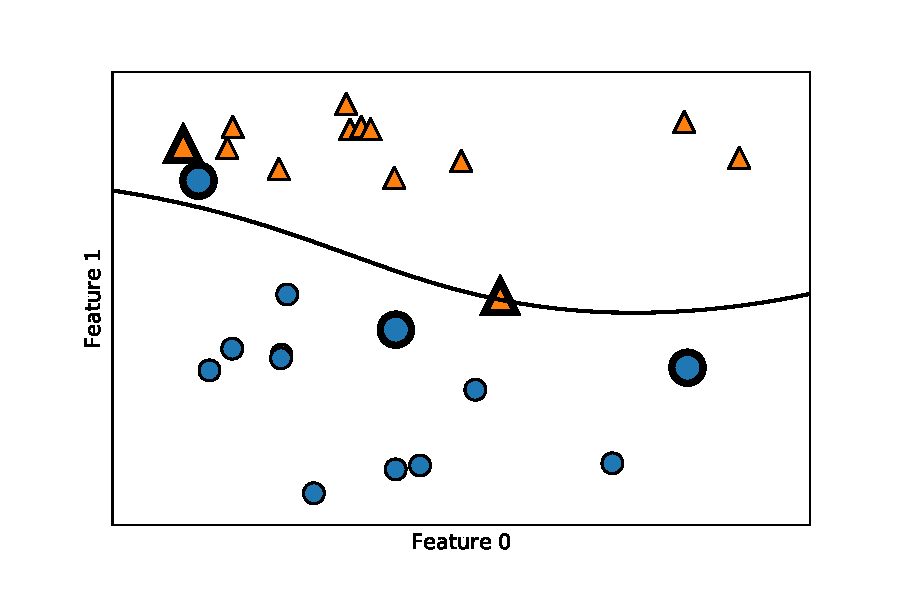
\includegraphics[width=\columnwidth]{images/Figure1.pdf}
  \caption{K-Nearest Neighbors Classifier Accuracy for Training Set and 
  Testing Set as a function of Number of Neighbors}
  \label{f:Figure1}
\end{figure}

%%%%%%%%%%%%%%%%%%%%%%%%%%%%%%%%%%%%%%%%%%%%%%%%%%%%%%%%%%%%%%%%%%%%%%%%%%%%%%%%
\subsubsection{Linear Classifier Models}

Logistic regression is a commonly used linear model for classification 
problems. The decision boundary for the logistic regression classifier is a 
linear function of the input; a binary classifier separates two classes using 
along a line, plane, or hyperplane. Linear classification models differ in 
terms of (1) how they measure how well a particular combination of coefficients 
and intercept fit the training data, and (2) the type of regularization used 
\cite{muller17}. The main parameter for linear classification models is the
regularization parameter C. High values of C correspond to less regularization 
and the model will fit the training set as best as possible, stressing the 
importance of each individual data point to be classified correctly. By 
contrast, with low values of C, the model puts more emphasis on finding 
coefficient vectors (i.e., weights) that are close to zero, trying to adjust to 
the majority of data points. In addition, the penalty parameter influences the 
coefficient values of the linear model. The L2 penalty (Ridge) uses all 
available features, but pushes the coefficient values toward zero. The L1 
penalty (Lasso) sets the coefficient values for most features to zero, and uses 
only a subset of features for improved interpretability. This analysis used a 
logistic regression classifier to predict Heroin use from demographic 
attributes, mental health, prescription opioids, medication use, misuse, 
and illicit drug use. 

%%%%%%%%%%%%%%%%%%%%%%%%%%%%%%%%%%%%%%%%%%%%%%%%%%%%%%%%%%%%%%%%%%%%%%%%%%%%%%%%
\subsubsection{Non-linear Classifier Models}

Support Vector Machines


Naive Bayes


Neural Networks

\begin{figure}[!ht]
  \centering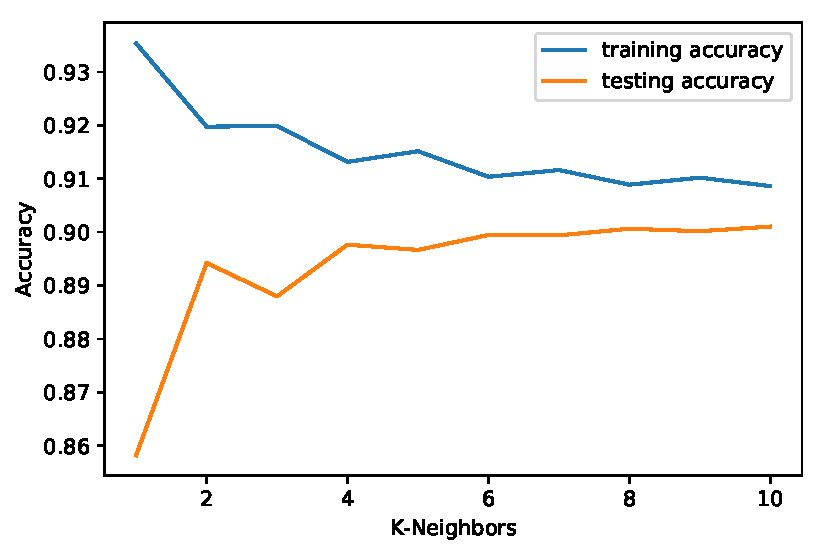
\includegraphics[width=\columnwidth]{images/Figure2.pdf}
  \caption{Neural Net Classifier: Multilayer Perceptron with Single Hidden Layer}
  \label{f:Figure2}
\end{figure}
%%%%%%%%%%%%%%%%%%%%%%%%%%%%%%%%%%%%%%%%%%%%%%%%%%%%%%%%%%%%%%%%%%%%%%%%%%%%%%%%

\subsubsection{Decision Tree Models}

Decision tree models are widely used for classification and regression. Tree 
models ``learn'' a hierarchy of if-else questions that are represented in the
form of a decision tree. Building decision trees proceeds from a root node as 
the starting point and continues through a series of decisions or choices.
Each node in the tree either represents either a question or a terminal node 
(i.e.,leaf) that contains the outcome. Applied to a binary classification task, 
the decision tree algorithm \emph{learns} the sequence of if-else questions 
that arrives at the outcome most quickly. For continuous features, the 
decisions are expressed in the form of, ``Is feature x larger than value y?''
 In constructing the tree the algorithm searches through all
possible decisions or tests and finds a solution that is most informative 
about the target outcome \cite{muller17}. A decision tree classifier is used 
for binary or categorical targets, and decision tree regression is used for 
continuous target outcomes. The recursive branching process of tree based 
models yields a binary tree of decisions, with each node representing a test 
that considers a single feature. This process of recursive partitioning is 
repeated until each leaf in the decision tree contains only a single target. 
Prediction for a new data point proceeds by checking which region of the 
partition the point falls in, and predicting the majority in that feature space. 
The main advantage of tree based models is that they require little adjustment 
and are easy to interpret. A drawback is that they can lead to complex models 
that are highly overfit to the training data. A common strategy to prevent 
overfitting is \emph{pre-pruning}, which stops tree construction early by 
limiting the maximum depth of the tree, or the maximum number of leaves. 
One can also set the minimum number of points in a node required for splitting. 
Another approach is to build the tree and then remove or collapse nodes with 
little information, which is called \emph{post-pruning}. Decision trees work 
well with features measured on very different scales, or with data that has 
a mix of binary and continuous features. 

%%%%%%%%%%%%%%%%%%%%%%%%%%%%%%%%%%%%%%%%%%%%%%%%%%%%%%%%%%%%%%%%%%%%%%%%%%%%%%%%
\subsubsection{Random Forests Classifier}

A random forest is a collection of decision trees that are slightly different 
from the others, which each overfits the data in different ways. The idea 
behind random forests is that overfitting can be reduced by building many 
trees and averaging their results. This approach retains the predictive power 
of trees while reducing overfitting. Randomness is introduced into the tree 
building process in two ways: (a) selecting a bootstrap sample of the data, 
and (b) selecting features in each node branch \cite{muller17,raschka17}. In 
building the random forest, we first decide how many trees to build (e.g., 10 
or 100), and the algorithm makes different random choices so that each tree is 
distinct. The bootstrapping method repeatedly draws random samples of size n 
from the dataset (with replacement). The decision trees are build on these 
random samples that are the same size as the original data, with some points 
missing and some data points repeated. The algorithm also selects a random 
subset of p features, repeated separately each node in the tree, so that 
each decision at the node branch is made using a different subset of features.
These two processes help ensure that all of the decision trees in the random
forest are different. 

The important parameters for the random forests 
algorithm are the number of sampled data points and the maximum number of 
features; the algorithm could look at all of the features in the dataset
or a limited number. A high value for \emph{maximum-features} will produce 
trees in the random forest that are very similar and will fit the data 
easily based on the most distinctive features, whereas a low value will 
produce trees that are very different from each other, and reduces over-
fitting. Random forests is of the most widely used ML algorithms that works 
well without very much parameter tuning or scaling of data. A limitation of 
this approach is that Random forests do not perform well with very high-
dimensional, data that is sparse data, such as text data.

\subsubsection{Gradient Boosted Tree Classifier}

%%%%%%%%%%%%%%%%%%%%%%%%%%%%%%%%%%%%%%%%%%%%%%%%%%%%%%%%%%%%%%%%%%%%%%%%%%%%%%%%

\subsection{Metrics for Evaluating Prediction Models}

Comparing the performance of different learning algorithms can be helpful for 
selecting the best model for a given problem. Binary classification is assessed 
in terms of the successful assignment of observations to one of two classes: 
positive or negative. In the present case, individuals are classified either 
as having misused and abused pain relievers or not. Model performance is 
commonly evaluated using accuracy which is defined by the number of correct 
predictions divided by the total number of all samples. Any model selected 
cannot make perfect predictions as there are always mistakes to be found. 
For example, a negative instance can be labeled as positive: a person who has 
never misused or abused pain relievers may be classified as having done so 
(i.e., 'false positive'). Conversely, a positive instance may be classified 
as negative: a person who has misused and abused pain relievers may be labeled 
as never having done so (i.e., 'false negative'). Table 1 shows the kinds of 
classification errors and correct decisions represented in a 
\emph{confusion matrix} which indicates the correspondence between predicted 
and actual outcomes. The confusion matrix is a two-by-two array in which the 
columns correspond to the actual observed classes and the rows correspond to 
the predicted classes. The main diagonal indicate the number of correctly 
classified samples (\emph{true positive, true negative}, while the other 
entries represent the number of samples in one class that were mistakenly 
classified as another class. Classification models are evaluated using several 
measures including recall, precision, and the $f_1$-score \cite{wiki18}. 
\emph{Recall} or ``sensitivity'' measures how many positive samples are 
captured by the positive predictions ( \(\frac{TP}{TP+FN}\) ), and is used 
when we want to identify all positive samples while avoiding false negatives. 
\emph{Precision} or the ``positive predictive value'', measures how many of 
the samples predicted as positive are actually positive 
( \(\frac{TP}{TP+FP}\) ), and is used as a metric when the goal is to limit 
the number of false positives. The \emph{$f_1$-score} or `f-measure' provides 
the harmonic mean of precision and recall. The $f_1$-score can be a better 
metric than accuracy in datasets with \emph{imbalanced classes}, where one 
class is much more frequent than the other class, as it takes recall and 
precision into account \cite{muller17}.

\begin{equation}
  \ f_1 score = 2*\frac{Precision*Recall}{Precision+Recall}\
\end{equation}

%%%%%%%%%%%%%%%%%%%%%%%%%%%%%%%%%%%%%%%%%%%%%%%%%%%%%%%%%%%%%%%%%%%%%%%%%%%%%%%%

\begin{table}
  \caption{Confusion Matrix for Evaluating Classification Model Performance}
  \label{tab:freq}
  \begin{tabular}{llll}
    \toprule
     &  &  Actual Outcome & \\
    \midrule
     Predicted & Outcome & No Misuse & PRL Misuse \\
    \midrule
     & No Misuse & \textbf{True Negative} & False Positive \\
    \midrule
     & PRL Misuse & False Negative & \textbf{True Positive} \\
    \bottomrule
  \end{tabular}
\end{table}

%%%%%%%%%%%%%%%%%%%%%%%%%%%%%%%%%%%%%%%%%%%%%%%%%%%%%%%%%%%%%%%%%%%%%%%%%%%%%%%%
\subsection{Project Goals} 

The main hypothesis is that pain reliever misuse and abuse (PRLMISAB) can be
predicted by demographic features, medication use, and use of illicit drugs. 

that prescription opioid dependency and
addicted will in many cases lead to the use of illicit opioids such as heroin 
or fentanyl. 
According to this reasoning, it was hypothesized that individuals 
who report using heroin may also be susceptible to misusing or abusing 
prescription opioid medications. 

The goal of the study was to identify the set 
of features important for predicting opioid addiction. The data used in the 
project is from the National Survey on Drug Use and Health from 2015 (NSHUH-
2015) \cite{samhsa16}, which is the most recent year available. The NSDUH-2015 
is a comprehensive survey that covers all aspects of substance use, misuse, 
dependency, and abuse, including questions related to both prescription 
medications (opioids, tranquilizers, sedatives) and illicit drugs (e.g., 
heroin, cocaine, methamphetamine), drug dependency, addiction, and treatment, 
demographic measures of education and employment, physical health, depression, 
and mental health treatment. Several classification models were constructed to 
classify heroin use in the sample by demographics attributes and mental health 
characteristics (e.g., adult depression). This method addresses the following
issues related to opioid dependency and addiction: (i) Identify factors related 
to illicit opioid use, (ii) Identify factors related to prescription opioid 
misuse and abuse, and (iii) Examine the relationship between prescription 
opioid misuse, abuse and heroin use. 


%%%%%%%%%%%%%%%%%%%%%%%%%%%%%%%%%%%%%%%%%%%%%%%%%%%%%%%%%%%%%%%%%%%%%%%%%%%%%%%%

\begin{table}
  \caption{Classification Models for Predict Pain Reliever Misuse 
  and Abuse and Main Parameters}
  \label{tab:freq}
  \begin{tabular}{ll}
    \toprule
    Model & Main Parameter \\
    \midrule
    K-Nearest Neighbors & Number of Neighbors = 4 \\
    Logistic Regression & Number of Features = 15 \\
    Linear Discriminant Analysis (LDA) & Number of Features = 15 \\
    Support Vector Machines (SVM) & Kernel = linear \\
    Naive Bayes & Cost C = 0.01 \\
    Neural Network & Hidden Layers = 2 \\
    Decision Trees & Tree-Depth = 4 \\ 
    Random Forests & Number of Trees = 100 \\
    Boosted Trees & Learning Rate = 0.01 \\ 
    \bottomrule
  \end{tabular}
\end{table}

%%%%%%%%%%%%%%%%%%%%%%%%%%%%%%%%%%%%%%%%%%%%%%%%%%%%%%%%%%%%%%%%%%%%%%%%%%%%%%%%
\section{Method}

The project workflow included the following steps: (1) Data download and 
extraction, (2) Data cleaning and preparation, (3) Exploratory data analysis 
and Visualization, (5) Construction and analysis of classification models of
prescription pain reliever misuse and abuse (PRLMA).

\subsection{Data Cleaning and Preparation }

All steps of data cleaning, preparation, and aggregation were completed using 
a python interactive notebook \cite{mckinney17}.

downloaded from the Substance Abuse and Mental 
Health Data Archive (SAMHDA) \cite{samhsa18}
After downloading the NSDUH 
data files for 2015 and 2016 as a data frame object,




The dataset consists 
of 57,146 observations with 2,666 features representing individual-level 
responses from a survey of the U.S. population.


Data from the 2015 NSHUH was  URL using the get-data.py 
function written to unzip the data files, extract the data as a Pandas data 
frame, and write the file to CSV file

all identifying information is collapsed (e.g., age categories), 
variables related to ethnicity, immigration status, and state identifiers 
are removed to ensure confidentiality.

obtained from the Substance Abuse and Mental Health 
Data Archive (SAMHDA) \cite{samhsa16}.

The weighted survey screening response rate was 81.94 percent and the weighted 
interview response rate was 71.2 percent. For the present study, approximately
90 variables were selected that were aggregated to a data set of 20 variables. 

As described in the NSDUH codebook, sampling was weighted across states by 
population size for a representative distribution selected from 6,000 area segments. 

According 
to the NSDUH codebook, sampling was weighted across states by population size 
for a representative distribution selected from 6,000 area segments. The sample 
design used five state sample size groups, drawing more heavily from the eight 



The dataset was split into the training set and test 
sets using the train-test-split function in sklearn and the target variables 
was designated. Model accuracy for the training set and test set are reported, 
for different parameter values, with feature importance. 


the 
dataset was subset by columns to include demographic characteristics (e.g., 
age category, sex, marital status, education, employment status, and category 
of metropolitan area), measures of physical health (e.g., overall health, 
STDs, Hepatitis, HIV, Cancer, hospitalization), mental health (e.g., Adult 
Depression, Emotional Distress, Suicidal Thoughts, Plans), Suicide Attempts, 
Pain Reliever Medication Use, Misuse, and Abuse (over past year, past month), 
Prescription Opioid Medications Taken in Past year (e.g., Hydrocodone, 
Oxycodone, Tramadol, Morphine, Fentanyl, Oxymorphone, Demerol, Hydromorphone), 
Heroin Use, Abuse (over past year, past month), Tranquilizer Use, Sedative Use, 
Cocaine Use, Amphetamine and Methamphetamine Use, Hallucinogen Use, Drug 
Treatment (e.g., Inpatient, Outpatient, Hospital, Mental Health Clinic, ER, 
Drug Treatment Status), and Mental Health Treatment History. A codebook was 
created to provide a complete list of variables included with summaries 
of response categories \cite{codebook17}. The following steps were taken 
to detect and remove inconsistencies in the data \cite{rahm00}:
\begin{enumerate}
  \item Remove missing values (i.e., NaN) 
  \item Recode blanks, non-responses, or legitimate skips (e.g., 99, 991, 
  993) to zero  
  \item Recode dichotomous responses (e.g., Yes=1 / No=2) so that No=0
  \item Recode categorical variables to be consistent with amount or degree 
  (e.g., 1=low, 2=med, 3=high)
   \item Rename selected variables for better description (e.g., 
   Adult Major Depressive Episode Lifetime changed from AMDELT to DEPMELT)
\end{enumerate}

%%%%%%%%%%%%%%%%%%%%%%%%%%%%%%%%%%%%%%%%%%%%%%%%%%%%%%%%%%%%%%%%%%%%%%%%%%%%%%%%
\subsubsection{Aggregated Variables}

Because the majority of features were represented as dichotomous Yes / No 
variables, related features were summed to create aggregated variables. For 
example, overall health, STD, Hepatitis, HIV, Cancer, and hospitalization were 
aggregated to create a single health measure. The health measure was recoded
so that higher scores indicated better health. Questions related to depression, 
emotional distress, and suicidal thoughts were summed to create a single 
variable for mental health (MENTHLTH) with scores ranging from 0 to 9. 
Responses to pain reliever medication use, misuse, abuse, or dependency, 
were aggregated to create a single variable of pain reliever misuse or abuse
(PRLMISAB). All prescription painkiller medications used in the past year
were summed. Similarly, all related responses were summed to create single 
variables for Tranquilizers, Sedatives, Cocaine, Amphetamines, Hallucinogens, 
Drug Treatment, and Mental Health Treatment. The target outcome of interest for 
classification, lifetime heroin use (i.e., ``Have you ever used heroin before, 
at any time?'') is a dichotomous variables. The demographic characteristics 
and aggregated variables were subset and saved to a new data frame consisting 
of 22 features and 57,146 observations, which was exported to CSV file. 

The features of interest were demographic 
characteristics, health, mental health (adultdepression), prescription 
opioid misuse and abuse (PRLMISEVR, PRLMISAB, PRLANY), prescription 
tranquilizers use and sedatives use (TRQLZRS, SEDATVS), use of illicit drugs 
(COCAINE, AMPHETMN), drug treatment (TRTMENT), and mental health treatment 
(MHTRTMT). 

"AGECAT"    "SEX"       "MARRIED"   "EDUCAT"    "EMPLOY18"  "CTYMETRO" 
"HEALTH"    "MENTHLTH"  "PRLMISEVR" "HEROINUSE" "TRQLZRS"   "SEDATVS"  
"COCAINE"   "AMPHETMN"  "TRTMENT"   "MHTRTMT"  

\begin{table*}[ht]
  \caption{Summary of Variables in the NSDUH 2015-16 Aggregated Data Set}
  \label{tab:freq}
  \begin{tabular}{ll}
    \toprule
    \textit{Dependent Variable} & Label \\
    \midrule
    Prescription Opioid Pain Reliever Misuse and Abuse (0-12 Scale)& PRLMISAB  \\
    \midrule
    \textit{Demographic Variables}&   \\
    \midrule
    Age Category (1=12-17 years, 2=18-25, 3=26-34, 4=35-49, 5=50 and older)& AGECAT \\
    Biological Sex (0=Male, 1=Female)& SEX  \\
    Marital Status (0=Unmarried, 1=Divorced, 2=Widowed, 3=Married)& MARRIED  \\
    Education (1=H.S. or Less, 2=H.S. Grad., 3=Some College,  4=College Grad.)& EDUCAT  \\
    Size of City/Metropolitan Region (1=Rural, 2=Small, 3=Large)& CTYMETRO  \\
    Health Problems Aggregated  (0-10 scale)& HEALTH  \\
    Mental Health, Aggregated: adult depression, emotional distress (0-10 scale)& MENTHLTH  \\
    Treatment for Drugs and Alcohol in past year, Aggregated (0-5 scale)& TRTMENT  \\
    Mental Health Treatment, Aggregated (Likert scale, 1-10)& MHTRTMT  \\
    \midrule
    \textit{Medication and Drug Use Variables}& \\
    \midrule
    Tranquilizer use, past year, Aggregated (Likert scale, 0-5)& TRQLZRS \\
    Sedative use, past year, Aggregated (0-5 scale)& SEDATVS  \\
    Heroin use, past year, Aggregated (0-5 scale)& HEROINUSE  \\
    Cocaine and Crack Cocaine Use in past year, Aggregated  (0-5 scale)& COCAINE  \\
    Amphetamine and Methamphetamine Use in past year, Aggregated (0-5 scale)& AMPHETMN  \\
    \bottomrule
  \end{tabular}
\end{table*}

%%%%%%%%%%%%%%%%%%%%%%%%%%%%%%%%%%%%%%%%%%%%%%%%%%%%%%%%%%%%%%%%%%%%%%%%%%%%%%%%
\section{Results}

\subsection{Exploratory Data Analysis}

The sample of N=57,146 respondents from 2015 (26,736 male, 30,410 female)
and N=57,146 respondents from 2016 (26,736 male, 30,410 female), resulting
in a total sample of N=57,146 respondents,

6,343 individuals reported misusing pain medication at some point
(3221 males, 3122 females), but only 956 respondents had used heroin (570 males, 
386 females). 

Of  26,736 were male and 30,410 
female; 6,343 individuals reported misusing pain medication at some point
(3221 males, 3122 females), but only 956 respondents had used heroin (570 males, 
386 females). 

Only few people 
self-described as high in depression reported low Prescription Opioid PRL 
misuse and abuse. 

 The target variable was Heroin Use (HEROINEVR). Next, 

%%%%%%%%%%%%%%%%%%%%%%%%%%%%%%%%%%%%%%%%%%%%%%%%%%%%%%%%%%%%%%%%%%%%%%%%%%%%%%%%

\subsection{Classification Models}

The dataset was divided into the training set and test set using a 75-25 
percent split. 


Each model was fit to the training set, new values were predicted and model 
performance was evaluated on the holdout scores in the test set. 

the train-test-split() function in sklearn. Model accuracy for the training 
set and test 
set are reported, with different parameter values, and features importance. 



\subsection{Comparison of Classifier Models}
 
Logistic Regression Classification is a based on a linear equation that 
calculates the relative weight of each feature for a categorical target or 
binary outcome (yes / no) \cite{raschka17}. The logistic regression classifier 
was fit to the training data in Scikit-Learn, and the model was validated on 
the test data. By default, the model applies L2 penalty (Ridge). The training 
set accuracy was 0.983 and the test set accuracy was 0.984. The parameter `C` 
determines the strength of regularization, with higher values of C providing
greater regularization. The L1 penalty (Lasso) limits the values of most 
coefficients to zero, creating a more interpretable model that uses only a 
few features. Figure 4 plots the coefficients of logistic regression classifier 
for heroin use with the L1 Penalty (Lasso) under different values of parameter 
C. The default setting, C=1.0, provides good performance for train and test 
sets, but the model is very likely underfitting the test data. Using a higher
value of C fits a more flexible model and generally gives improved accuracy 
for both training and tests sets. Using a value of C=100 yielded training set
accuracy of 0.98 and test set accuracy of 0.98. Figure 4 shows that the 
features coefficient values did not change much according to the values of
parameter C, and the accuracy values were approximately the same for all 
values of C. Examination of the coefficients from the logistic regression 
classifier revealed the three features which were most closely associated 
with Heroin use were: Prescription Opioid Pain Reliever (PRL) Misuse ever 
(as predicted), Cocaine Use, and Amphetamine use, respectively.





\begin{table*}[ht]
  \caption{Confusion Matrices and Performance Metrics for Predictive Models of Pain Reliever Misuse and Abuse}
  \label{tab:freq}
  \begin{tabular}{llllllll}
    \toprule
    Model& & Confusion Matrix & & Accuracy & Recall & Precision & F1-Score \\
    \midrule
    K-Nearest Neighbors Classifier & & No Misuse & PRL Misuse &  &  &  & \\
     & No Misuse & 25114 & 320 & 89.5\% & 0.900 & 0.870 & 0.870 \\
     & PRL Misuse & 2609 & 467 &  &  &  & \\
    \midrule
    Logistic Regression & & No Misuse & PRL Misuse &  &  &  & \\
     & No Misuse & 25002 & 2509 & 90\% & 0.986 & 0.909 & 0.946 \\
     & PRL Misuse & 344 & 654 &  &  &  & \\
    \midrule
    Linear Discriminant Analysis  & & No Misuse & PRL Misuse &  &  &  & \\
     & No Misuse & 24667 & 2238 & 89.8\% & 0.973 & 0.917 & 0.944 \\
     & PRL Misuse & 679 & 925 &  &  &  & \\
    \midrule
    Support Vector Classifier  & & No Misuse & PRL Misuse &  &  &  & \\
     & No Misuse & 25201 & 233 & 90.4\% & 0.900 & 0.890 & 0.880 \\
     & PRL Misuse & 2514 & 562 &  &  &  & \\
    \midrule
    Naive Bayes Classifier & & No Misuse & PRL Misuse &  &  &  & \\
     & No Misuse & 25345 & 3133 & 89\% & 0.999 & 0.890 & 0.941 \\
     & PRL Misuse & 1 & 30 &  &  &  & \\
    \midrule
    Neural Net (MLP) & & No Misuse & PRL Misuse &  &  &  & \\
     & No Misuse & 25088 & 346 & 90.6\% & 0.910 & 0.890 & 0.880 \\
     & PRL Misuse & 2366 & 710 &  &  &  & \\
    \midrule
    Decision Trees & & No Misuse & PRL Misuse &  &  &  & \\
     & No Misuse & 25042 & 2572 & 89.9\% & 0.988 & 0.907 & 0.946 \\
     & PRL Misuse & 304 & 591 &  &  &  & \\
    \midrule
    Random Forests & & No Misuse & PRL Misuse &  &  &  & \\
     & No Misuse & 25054 & 2518 & 90.1\% & 0.989 & 0.909 & 0.947 \\
     & PRL Misuse & 292 & 645 &  &  &  & \\
    \midrule
    Gradient Boosted Trees & & No Misuse & PRL Misuse &  &  &  & \\
     & No Misuse & 25415 & 19 & 89.6\% & 0.900 & 0.890 & 0.850 \\
     & PRL Misuse & 2954 & 122 &  &  &  & \\
    \bottomrule
  \end{tabular}
\end{table*}


%%%%%%%%%%%%%%%%%%%%%%%%%%%%%%%%%%%%%%%%%%%%%%%%%%%%%%%%%%%%%%%%%%%%%%%%%%%%%%%%
\subsubsection{Decision Tree Classifier}

The following analysis used the \emph{Decision Tree Classifier} package in 
Scikit-Learn, which only does pre-pruning. First, the decision model was build
using the default setting of a fully developed tree until all leaves are pure. 
The random state` features is fixed to break ties internally. Accuracy on the
training set was 0.99 and test set accuracy was 0.974. Without restricting 
their depth, decision trees can become complex; unpruned trees are prone to 
overfitting and do not generalize well to new data. Limiting the depth of 
tree decreases overfitting, which results in lower training set accuracy, 
but improved performance on the test set. 

Next, pre-pruning was applied, with 
a maximum depth of 4, which means the algorithm split on four consecutive
questions. Training set accuracy of the pruned tree was 0.985 and test set
accuracy was 0.984. Even with a depth of 4, the tree can become a bit complex.
Figure 5 shows a partial view of the decision tree classifier of heroin use 
(the entire tree was too wide to include as a legible Figure), and the full 
tree image is available in the notebook BDA-Analytics-Classifier-Heroin.ipynb 
\cite{classifyH}. 

The decision tree shows the top features that the algorithm 
split on to classify heroin use. One way to interpret a decision tree it by 
following the sample numbers represented at the test split for each node. 
The classifier algorithm selected Cocaine Use (aggregated score) as the root 
node of the decision tree. The branch to the left  side of the tree represents 
samples with a score equal to or less than 1.5 (n=40956), whereas the branch 
to the right represents samples with a Cocaine Use score greater than 1.5
(n=1903). The second split on the right occurs for Any Prescription Opioid 
Pain Reliever Use (PRLANY), with n=1443 having a score less than or equal 
to 3.5, and n=460 respondents with a PRL score greater than 3.5. In other 
words, of those respondents who reported relatively high Cocaine use, a small
portion also reported relatively high Prescription Opioid PRL use. Instead of 
looking at the whole tree, features importance is a common summary function 
that rates how important each feature is for the classification decisions 
made in the algorithm. Each feature is assigned an importance value between 
0 and 1; with a value of 1 indicating the feature perfectly predicts the 
target and a value of 0 meaning that the feature was not used at all. 
Feature importance values also always sum to 1. A feature may have a low 
feature importance value because another feature encodes the same information. 
The top two important features for classifying Heroin Use were Cocaine Use 
and Any Prescription Opioid PRL Use, with smaller importance given to Opioid 
PRL Misuse Ever and Prescription Opioid PRL Misuse and Abuse. 

The Decision Tree Classifier package in Scikit-Learn was used to build the 
tree model, pre-pruning was applied with a maximum depth of 4, which means 
the algorithm split on four consecutive questions. The training set accuracy 
of the pruned tree was 0.902 and test set accuracy was 0.902. Figure 9 shows 
a partial view of the decision tree classifier of prescription opioid misuse
(the full tree is included in the BDA-Analytics-Classifier-PRL.ipynb 
notebook) \cite{classifyPRL}. 

As Figure 9 shows, the decision tree classifier
selected Cocaine Use as the root note, that branched by the test score equal
to or less than 0.5 (any Cocaine Use). At the second node, on the branch to 
the right n=5015 samples were further divided according to heroin use, with 
n=1913 having a score greater than 0.5 (any Heroin Use). At the third node
on the right branch, samples were selected according to Tranquilizer
medication use, with n=1419 scoring positively. On the left branch, the 
second node selected was Drug Treatment, with n=2844 respondents scoring
positively that they had received Drug Treatment. Feature importance of
the decision tree classifier selected Cocaine Use as the most informative
feature for Prescription Opioid PRL Misuse. Following afterwards, 
Tranquilizer Use, Drug Treatment, and Heroin Use were tied for second place. 


%%%%%%%%%%%%%%%%%%%%%%%%%%%%%%%%%%%%%%%%%%%%%%%%%%%%%%%%%%%%%%%%%%%%%%%%%%%%%%%%
\subsubsection{Random Forests Classifier}

Random forests is an ensemble approach that builds many trees and averages 
their results to reduce overfitting. The model was build using the 
\emph{Random Forest Classifier} package in Scikit-Learn. The parameters of 
interest for building random forests are: (a) the number of trees 
(n-estimators), (b) the number of data points for bootstrap sampling 
(n-samples), and (c) the maximum number of features considered at each node 
(max-features). The max-features parameter determines how random each tree is, 
with smaller values of max-features resulting in trees in the random forest 
that are very different from each other. This analysis applied a random forest 
consisting of 100 trees to classify Heroin Use, and the random state was set to 
zero. The training set accuracy was 0.999 and the test set accuracy was 0.984. 
Often the default settings for random forests work well, but we can apply
pre-pruning as with a single tree, or adjust the maximum number of features. 
Feature importance for random forests is computed by aggregating the feature 
importance over trees in the random forest, and random forests gives
non-zero importance to more features than a single tree. Typically random
forests provide a more reliable measure of feature importance than the
feature importance for a single tree. Figure 6 shows the feature importance 
of the random forests classifier for heroin use with 100 trees. Similar to
the single tree, the random forest selected Cocaine Use as the most
informative feature in the model, followed by Any PRL Use, which is an 
aggregated measure of prescription opioid medication use. Following after 
that, several features were tied for third place of importance, namely 
Education Level, Overall Health, Age Category, and Pain Reliever Misuse 
and Abuse. Random forests provides much of the same benefit as decision
trees, while compensating for some of their shortcomings of overfitting.
Single trees are still useful for visually representing the decision process.

\begin{figure}[!ht]
  \centering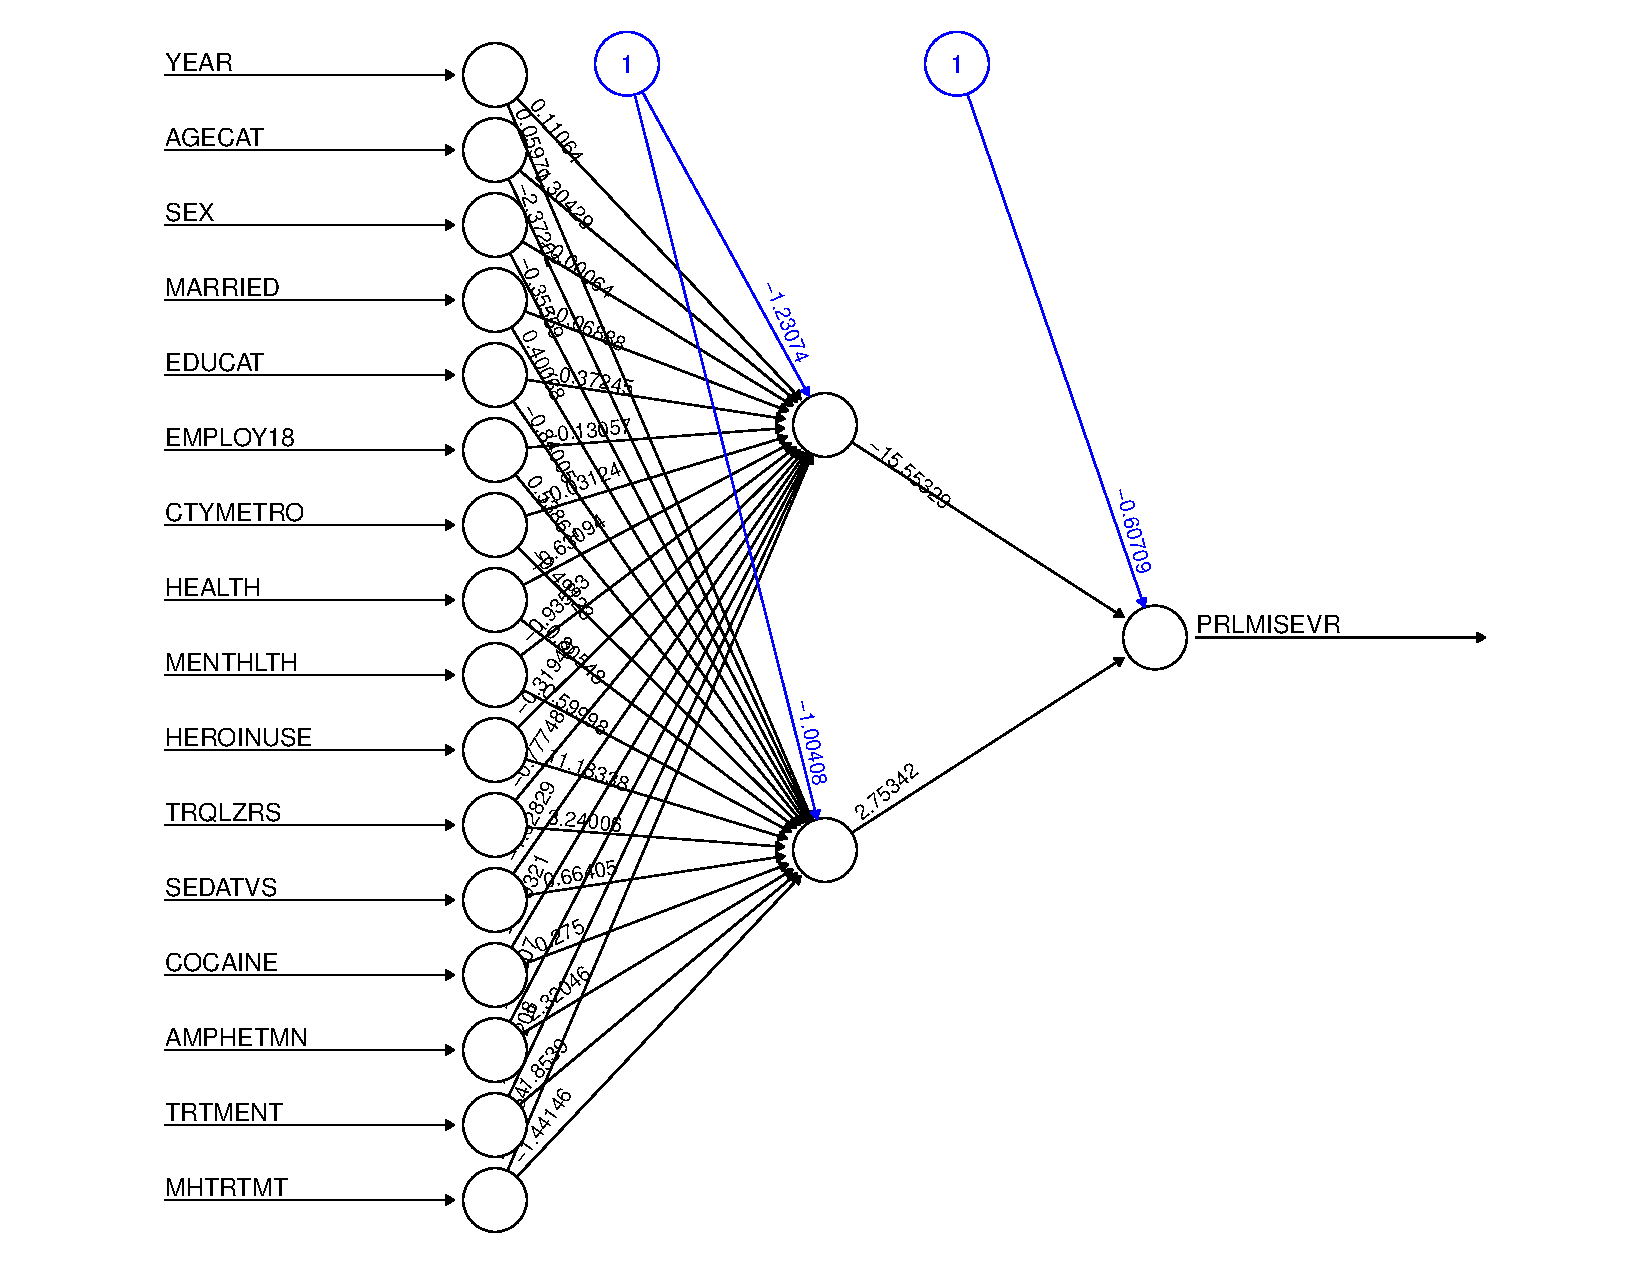
\includegraphics[width=\columnwidth]{images/Figure5.pdf}
  \caption{Decision Tree Classification of Heroin Use (Partial View)}
  \label{f:Figure5}
\end{figure}

%%%%%%%%%%%%%%%%%%%%%%%%%%%%%%%%%%%%%%%%%%%%%%%%%%%%%%%%%%%%%%%%%%%%%%%%%%%%%%%%
\subsubsection{Random Forests Classifier}

The Random Forest Classifier package in Scikit-Learn was used to classify
Prescription Opioid PRL Misuse as the target variable, with 100 trees. The 
model accuracy for the training set was 0.955 and the test set accuracy was 
0.896, which suggests that the model overfit the data. Figure 10 shows the 
feature importance of the random forests classifier for Prescription Opioid 
PRL Misuse. As Figure 10 shows, several features were identified as important
for classifying Prescription Opioid PRL Misuse. The random forest selected 
Overall Health as the most informative feature in the model, followed by 
Cocaine Use, Education Level, Age Category, and Size of City Metropolitan 
region. Because of the additional features included as important, gradient 
boosting was performed to clarify the feature importance.
%%%%%%%%%%%%%%%%%%%%%%%%%%%%%%%%%%%%%%%%%%%%%%%%%%%%%%%%%%%%%%%%%%%%%%%%%%%%%%%%
\subsubsection{Gradient Boosting Classifier Tree}

Gradient boosting machines is another ensemble method that combines multiple
decision trees for regression or classification by building trees in a serial 
fashion, where each tree tries to correct for mistakes of the previous one
\cite{muller17}. Gradient boosted regression trees use strong pre-pruning, 
with shallow trees of a depth of one to five. Each tree only provides a good
estimate of part of the data, but combining many shallow trees (i.e., ``weak 
learners''), the use many simple models iteratively improves performance. In 
addition to pre-pruning and the number of trees, an important parameter for 
gradient boosting is the learning rate, which determines how strongly each
tree tries to correct for mistakes of previous trees. A high learning rate
produces stronger corrections, allowing for more complex models. Adding
more trees to the ensemble also increases model complexity. Gradient boosting
and random forests perform well on similar tasks and data; it is common to
first try random forests and then include gradient boosting to attain 
improvements in accuracy of the learning model. This analysis used the 
\emph{Gradient Boosting Classifier} from Scikit-Learn to classify Heroin Use, 
with the default setting of 100 trees of maximum depth of 3, and a learning 
rate of 0.1. The model was build on the training set and evaluated on the test 
set, with both training set and test set accuracy equal to 0.984. To reduce
overfitting, pre-pruning could be implemented by reducing the maximum depth, 
or by reducing the learning rate. Figure 7 shows that the feature importance 
for the gradient boosting classifier tree looks similar to the feature 
importance for random forests, but the gradient boosting has decreased the 
importance of many features to zero. Again Cocaine is selected as the most 
imformative features, followed by Any Opioid PRL Use. In addition to 
Prescription Opioid PRL Misuse and Abuse, the gradient boosting classifier 
selected Amphetamine Use as an informative feature of Heroin Use. 

\begin{figure}[!ht]
  \centering\includegraphics[width=\columnwidth]{images/Figure7.pdf}
  \caption{Feature Importance for Gradient Boosting Classifier for Heroin Use}
  \label{f:Figure7}
\end{figure}

The Gradient Boosting Classifier from Scikit-Learn was used to classify 
Prescription Opioid PRL Misuse, using the default setting of 100 trees, of 
maximum depth of 3, and a learning rate of 0.1. The model accuracy for the
training set was 0.894 and accuracy for the test set was 0.893. Gradient 
boosting typically improves test set accuracy by using many simple models 
iteratively. In this case, model accuracy for gradient boosting was no better 
than random forests, and this is because the default parameter settings were
used; further parameter tuning is needed to improve model performance. Feature 
importance was a primary interest for identifying features related to '
prescription opioid abuse. Figure 11 shows the feature importance for the 
gradient boosting classifier tree. As Figure 11 shows, several features were 
important for classifying prescription opioid misuse, and contrary to the 
random forests, gradient boosting selected Tranquilizer use as the most 
informative feature. Following closely in importance were Heroin Use and Age 
Category. Tied for fourth place were Cocaine Use and Treatment, with Mental 
Health (depression) coming in fourth in terms of feature importance. This 
result illustrates that several features are important for understanding 
Prescription Opioid Misuse, and the relations among features may be complex.



%%%%%%%%%%%%%%%%%%%%%%%%%%%%%%%%%%%%%%%%%%%%%%%%%%%%%%%%%%%%%%%%%%%%%%%%%%%%%%%%

\section{DISCUSSION}

The results show that rates of prescription opioid use, misuse, and abuse are
much higher than use of illicit opioids such as heroin and fentanyl. The use 
of Hydrocodone (Vicodan) was double the rate of Oxycodone use (Oxycodone) 
across almost all age groups. The use of traditional prescription opioids 
was greater than reported use of synthetic opioids. Illicit drug use was 
highest for respondents between the ages of 18 to 25. In terms of mental 
health, more individuals between 18 to 25 years reported experiencing a major 
depressive episode (in adulthood) than any other age group. In terms of the 
so-called \emph{treatment gap}, almost twice as many respondents between 
18 to 25 years who felt a need for substance use treatment, had not received
treatment, than younger individuals between 12 to 17 years. The large majority 
of respondents (approximately 90 percent) had not misused prescription opioid 
pain relievers or used heroin. However, of those individuals who reported 
misusing prescription opioid pain relievers, almost twice as many had also
used heroin than had not (see Figure 1), which partially supports the 
hypothesis that prescription opioid use is associated will use of illicit 
opioids such as heroin. Prescription opioid misuse and heroin use was also
higher in large metropolitan areas than smaller cities or rural areas, but
a small portion of individuals in non-metropolitan regions reported very
high levels of prescription opoioid misuse. These data points may represent 
outliers, but a large sample would allow for analysis of how opioid misuse 
and addiction differ for smaller rural regions versus large urban areas. 

%%%%%%%%%%%%%%%%%%%%%%%%%%%%%%%%%%%%%%%%%%%%%%%%%%%%%%%%%%%%%%%%%%%%%%%%%%%%%%%%

\subsection{Comparison of Classifier Models}

Several classifier algorithms were used to identify relevant features for 
predicting heroin use and prescription opioid misuse. Comparing the performance 
of different algorithms is helpful for  selecting the best model. Test set
accuracy was comparable across models for both Heroin Use (0.98) and 
Prescription Opioid PRL Misuse (0.89-0.90). Logistic Regression provided the
feature coefficients for different values of the regularization parameter C. 
The Decision Tree classifier provided a easy to use, interpretable visual of
the decisions involved at each step of classification. Random forests provides
a more reliable indication of features importance than a single tree, 
whereas the gradient boosting classifier included additional tuning 
parameter for a more powerful model and more interpretable analysis of
feature importance. Each classifier method provides a different level of
analysis. For classifying heroin use, the logistic regression classified
showed that Prescription Opioid PRL Misuse had the highest coefficient value, 
but the tree-based classifiers each identified Cocaine Use as the most
informative feature for predicting heroin use. For classifying Prescription 
Opioid PRL Misuse, logistic regression showed that Treatment had the highest
coefficient value, but the tree based models each differed in selecting the
most important features. Decision trees indicated that Cocaine Use was most
informative, the random forests classifier selected health as the most
important feature, and the gradient boosting model selected Tranquilizer use
as most informative of prescription opioid PRL misuse. The different model 
each have their advantages and limitations, logistic regression provides the
coefficients, but random forests and gradient boosting are helpful for 
identified sets of important features.

%%%%%%%%%%%%%%%%%%%%%%%%%%%%%%%%%%%%%%%%%%%%%%%%%%%%%%%%%%%%%%%%%%%%%%%%%%%%%%%%
\subsection{Limitations}

Surveys data may be biased to some degree, but measures of confidentiality and 
anonymity help to assure more accurate disclosures. 

The main goal of this project was to identify features relevant for predicting 
opioid addiction by classifying cases according to heroin use. Only a small 
proportion of the sample reported having used heroin, and scores for mental
health issues were very low. A limitation of survey data is that responses may 
be biased by under-reporting or minimizing the use of illicit or illegal 
substances. People may also be reluctant to disclose mental health issues or 
health problems (e.g., STDs, HIV status, suicide attempts). It is possible
that this sample is representative of the frequency of opioid use and misuse
in the larger population. Recent statistics from the CDC show that heroin use
has increased among most demographics groups, with an average estimated rate 
of approximately 2.6 percent between 2011-2013 \cite{cdc16}. The rate of heroin 
use reported in the NSDUH-2015 sample was 1.6 percent. Therefore, it seems
that the actual rate of heroin use in the U.S. population may not be accurately
reflected in this sample. Another limitation is that the project dataset was 
constructed as a subset of features from the NSDUH-2015 data. Ninety 
attributes were selected out of 2666 features in the original dataset, and many 
features were combined to create aggregated variables for health, mental 
health, prescription opioid misuse and abuse, drug treatment, mental health
treatment. Future research could include a more comprehensive selection of
features to identify the set of features relevant for predicting opioid
dependency and addiction. An important challenge for making sense of big data 
is developing analytic tools adequate to handle large volumes of data.


%%%%%%%%%%%%%%%%%%%%%%%%%%%%%%%%%%%%%%%%%%%%%%%%%%%%%%%%%%%%%%%%%%%%%%%%%%%%%%%%
\subsection{Extension to Big Data}

A general tenet of big data is that, ``More data is always better.'' The 
methods used in this project could be extended to better approximate big data 
for predicting opioid use in the following ways: (1) Include a larger 
selection of features from the attributes in the NSDUH-2015 dataset; (2) 
Include survey data from previous years (e.g., 2005-2015) for a larger sample;  
and (3) Obtain a broader sample from the population of patients who are 
taking prescribed opioid medications. The most immediate step would be to 
include additional features for use with the classifier models. Additional 
data from the NSDUH was downloaded from previous years (2012 to 2014); 
preliminary examination of the data revealed inconsistencies in questions 
and prescription opioid medications that would need to be resolved in order 
to combine data from multiple years. Data cleaning can be a time consuming 
process, but important for obtaining usable data. Unfortunately, owing to 
constraints of time for completing the project, it was not possible to
integrate data from previous years into the project dataset. In working with
big data, there are there are several steps involved in the consolidation of 
data from multiple sources into a single dataset (in addition to data 
cleaning), which include extraction, integration, and aggregation of features  
\cite{rahm00}. A future study could integrate data from different years, 
using a broader set of features, with more inclusive sample representative
of the larger population, and integrate data from multiple sources. 

%%%%%%%%%%%%%%%%%%%%%%%%%%%%%%%%%%%%%%%%%%%%%%%%%%%%%%%%%%%%%%%%%%%%%%%%%%%%%%%%
\subsection{Opioid Addiction and Epidemic Spreading}

Drug addiction has many similar characteristics to other chronic medical 
illnesses, but there are unique challenges to the treatment of addiction
\cite{marsch12, swendson16}. In drug rehabilitation treatment programs, 
patients undergo intense detoxification that reduces their drug tolerance, 
but are then released back into the environments associated with their drug 
use, putting them at high risk for relapse and potential drug overdose 
\cite{johnson11}. If the prescription opioid crisis is a genuine epidemic, 
we must consider the process of spreading or diffusion of contagion. Epidemic 
spreading is a dynamic process based on networks of direct person-to-person 
contact and indirect exposure via transportation pathways \cite{Colizza06}. 
Epidemics are quantified in terms of the proportion of the population infected, 
those yet to be infected, and the rate of transmission. Potentially everyone
is at risk of becoming dependent or addicted to prescription medications or 
illicit opioids. In terms of the opioid epidemic, rather than labeling persons 
as infected or uninfected, it is more useful to consider people as either 
susceptible to dependence and addiction or less susceptible. Furthermore, 
the structure of the contact network can influence epidemic spreading
\cite{pastor01}. For example, in the case of simple contagion, weak 
ties among acquaintances or infrequent associations provide shortcuts between 
distant nodes that reduce distance within the network \cite{granovetter73} 
which can facilitate the spread of contagion, or in this case drug use. 
Furthermore, contact networks for drug use may have ``small world'' properties
where a small number of nodes have a high number of connection that can 
rapidly transmit contagion throughout the network \cite{watts98}. Network 
analysis may help to identify the underlying structure of the contact network
of opioid use, to examine pathways and points of contact in the misuse and 
abuse of prescription opioid medications. According to a classical conditioning
model of addiction, situational cues or events can elicit a motivational state 
underlying relapse to drug use. Addictive behavior can be also be reinstated 
after extinction of dependency by exposure to drug-related cues or stressors 
in the environment \cite{shaham03}. Future research could use social network 
modeling to explore how drug dependency and addiction are subserved by patterns 
of social interaction. 

%%%%%%%%%%%%%%%%%%%%%%%%%%%%%%%%%%%%%%%%%%%%%%%%%%%%%%%%%%%%%%%%%%%%%%%%%%%%%%%%
\section{Conclusion}

This project compared several classification algorithms to predict heroin use 
and prescription opioid misuse and abuse. The results provided partial support
for the hypothesis that prescription opioid misuse is associated with the use
of illicit opioids such as heroin. Several features were identified as 
important for classifying heroin use, including Cocaine Use, Amphetamine Use, 
and any prescription opioid medication use. In regards to predicting heroin
use, it appears the use of other illicit drugs such as Cocaine and Amphetamine 
was perhaps more informative than any prescription opioid use or misuse. Heroin 
use was selected as important for classifying prescription opioid pain reliever 
misuse, but additional factors also played as role, including tranquilizer use,
age category, overall health, cocaine use. Substance treatment had the largest
regression coefficient, suggesting that people who are misusing prescription
opioid pain medication are also more likely to be in drug treatment programs. 
The direction of these effects cannot be determined owing to the nature of the 
analyses. On the one hand individual misusing or abusing prescription opioids 
may also be using heroin. Alternatively, individuals with a susceptability for 
opioid use may be equally likely to have use heroin and also to have misused 
prescription opioids. A general conclusion is that of those individuals who 
reported misusing prescription opioid medications, twice as said they had used
heroin than reported they had not used heroin. The results do not provide 
sufficient evidence to rule out alternative hypotheses. Given the relatively 
low rates of opioid and heroin in this sample, additional evidence is needed to 
resolve this question. The study can provide information to raise awareness 
about the risk factors for prescription opioid addiction and may help reduce 
opioid overdose deaths. 




%%%%%%%%%%%%%%%%%%%%%%%%%%%%%%%%%%%%%%%%%%%%%%%%%%%%%%%%%%%%%%%%%%%%%%%%%%%%%%%%
\begin{acks}

Portions of this paper were completed as part of a course project in Big Data 
Applications and Analytics taugt by Dr. Gregor von Laszewskin at Indiana 
University in the Fall 2017. Thanks to the Professor von Laszewski and the
Teaching Assistants, Juliette Zurick, Miao Jiang, Hungri Lee, Grace Li, and 
Saber Sheybani Moghadam for helpful comments and feedback.

\end{acks}

\bibliographystyle{unsrt} %%ACM-Reference-Format%%
\bibliography{report} 


%%%%%%%%%%%%%%%%%%%%%%%%%%%%%%%%%%%%%%%%%%%%%%%%%%%%%%%%%%%%%%%%%%%%%%%%%%%%%%%%
\appendix

\section{Code References}
All code, notebooks, files, and folders for this project can be found in the

%%%%%%%%%%%%%%%%%%%%%%%%%%%%%%%%%%%%%%%%%%%%%%%%%%%%%%%%%%%%%%%%%%%%%%%%%%%%%%%%


%\input{issues}

\end{document}
